\documentclass{article}
\usepackage{spconf,amsmath,epsfig, amssymb}
\usepackage{subfigure}
\usepackage{multirow}

\def\x{{\mathbf x}}
\def\L{{\cal L}}

\title{Multi Target Video Tracking Using Residual Vector Quantization}
\name{Salman Aslam, Christopher Barnes, Aaron Bobick}
\address{Georgia Institute of Technolgy}
\begin{document}
\maketitle


%--------------------------------------------------------------------------------------------------------------------------------------
\begin{abstract}
%--------------------------------------------------------------------------------------------------------------------------------------
In this paper, we use Residual Vector Quantization (RVQ) for multi-target tracking.  To the best of our knowledge, this is the first reported application of RVQ to any form of video processing.  We implement a completely automatic method of initializing RVQ encoder and decoder codebooks from targets in a crowded scenario, and then use those codebooks to subsequently detect and track targets.
\end{abstract}

\begin{keywords}
Multi-target tracking, residual vector quantization, $\sigma$-tree classifier, pattern recognition, machine learning, source coding, compression.
\end{keywords}


%=============================================================================================================================
\section{INTRODUCTION}
%=============================================================================================================================
Multi-target tracking is one of the most complex tasks in video analytics.  In many cases, it is the first step in more complex processing tasks, such as temporal recognition and classification.  Many researchers have worked in this area.  
%--------------------------------------------------------------------------------------------------------------------------------------
\subsection{$\sigma$-tree Classifier and Residual Vector Quantization}
%--------------------------------------------------------------------------------------------------------------------------------------
\begin{figure}[t]
	\centering
	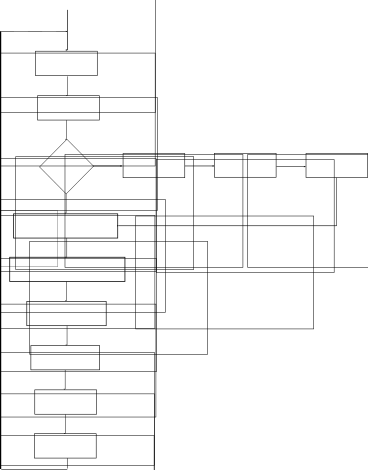
\includegraphics[width=0.45\textwidth]{figs/RVQ_TRK_IPCV2010_BlockDiagram}
	\caption{Block diagram.} 	
	\label{fig:block_diagram}	
\end{figure}

In this paper, we use the Image Driven Data Mining approach (IDDM )introduced in \cite{2007_JNL_IDDM_Barnes}.  This approach is based on the $\sigma$-tree for data warehouse similarity searching within the pixel-block space of feature classes, and for extracting labels from knowledge base collections or "aggregates".  These collections, in this paper are foreground blobs corresponding to tracked targets.  A key difference is that the data warehouse is built on-line, and is updated every few frames as new observations of the targets under interest arrive.  Another difference is that temporal correlations are used for unsupervised learning of target labels.  To better understand the $\sigma$-tree classifier, we relate it with five well-known areas of information theory, pattern recognition and machine learning.  

\begin{figure*}
	\centering
	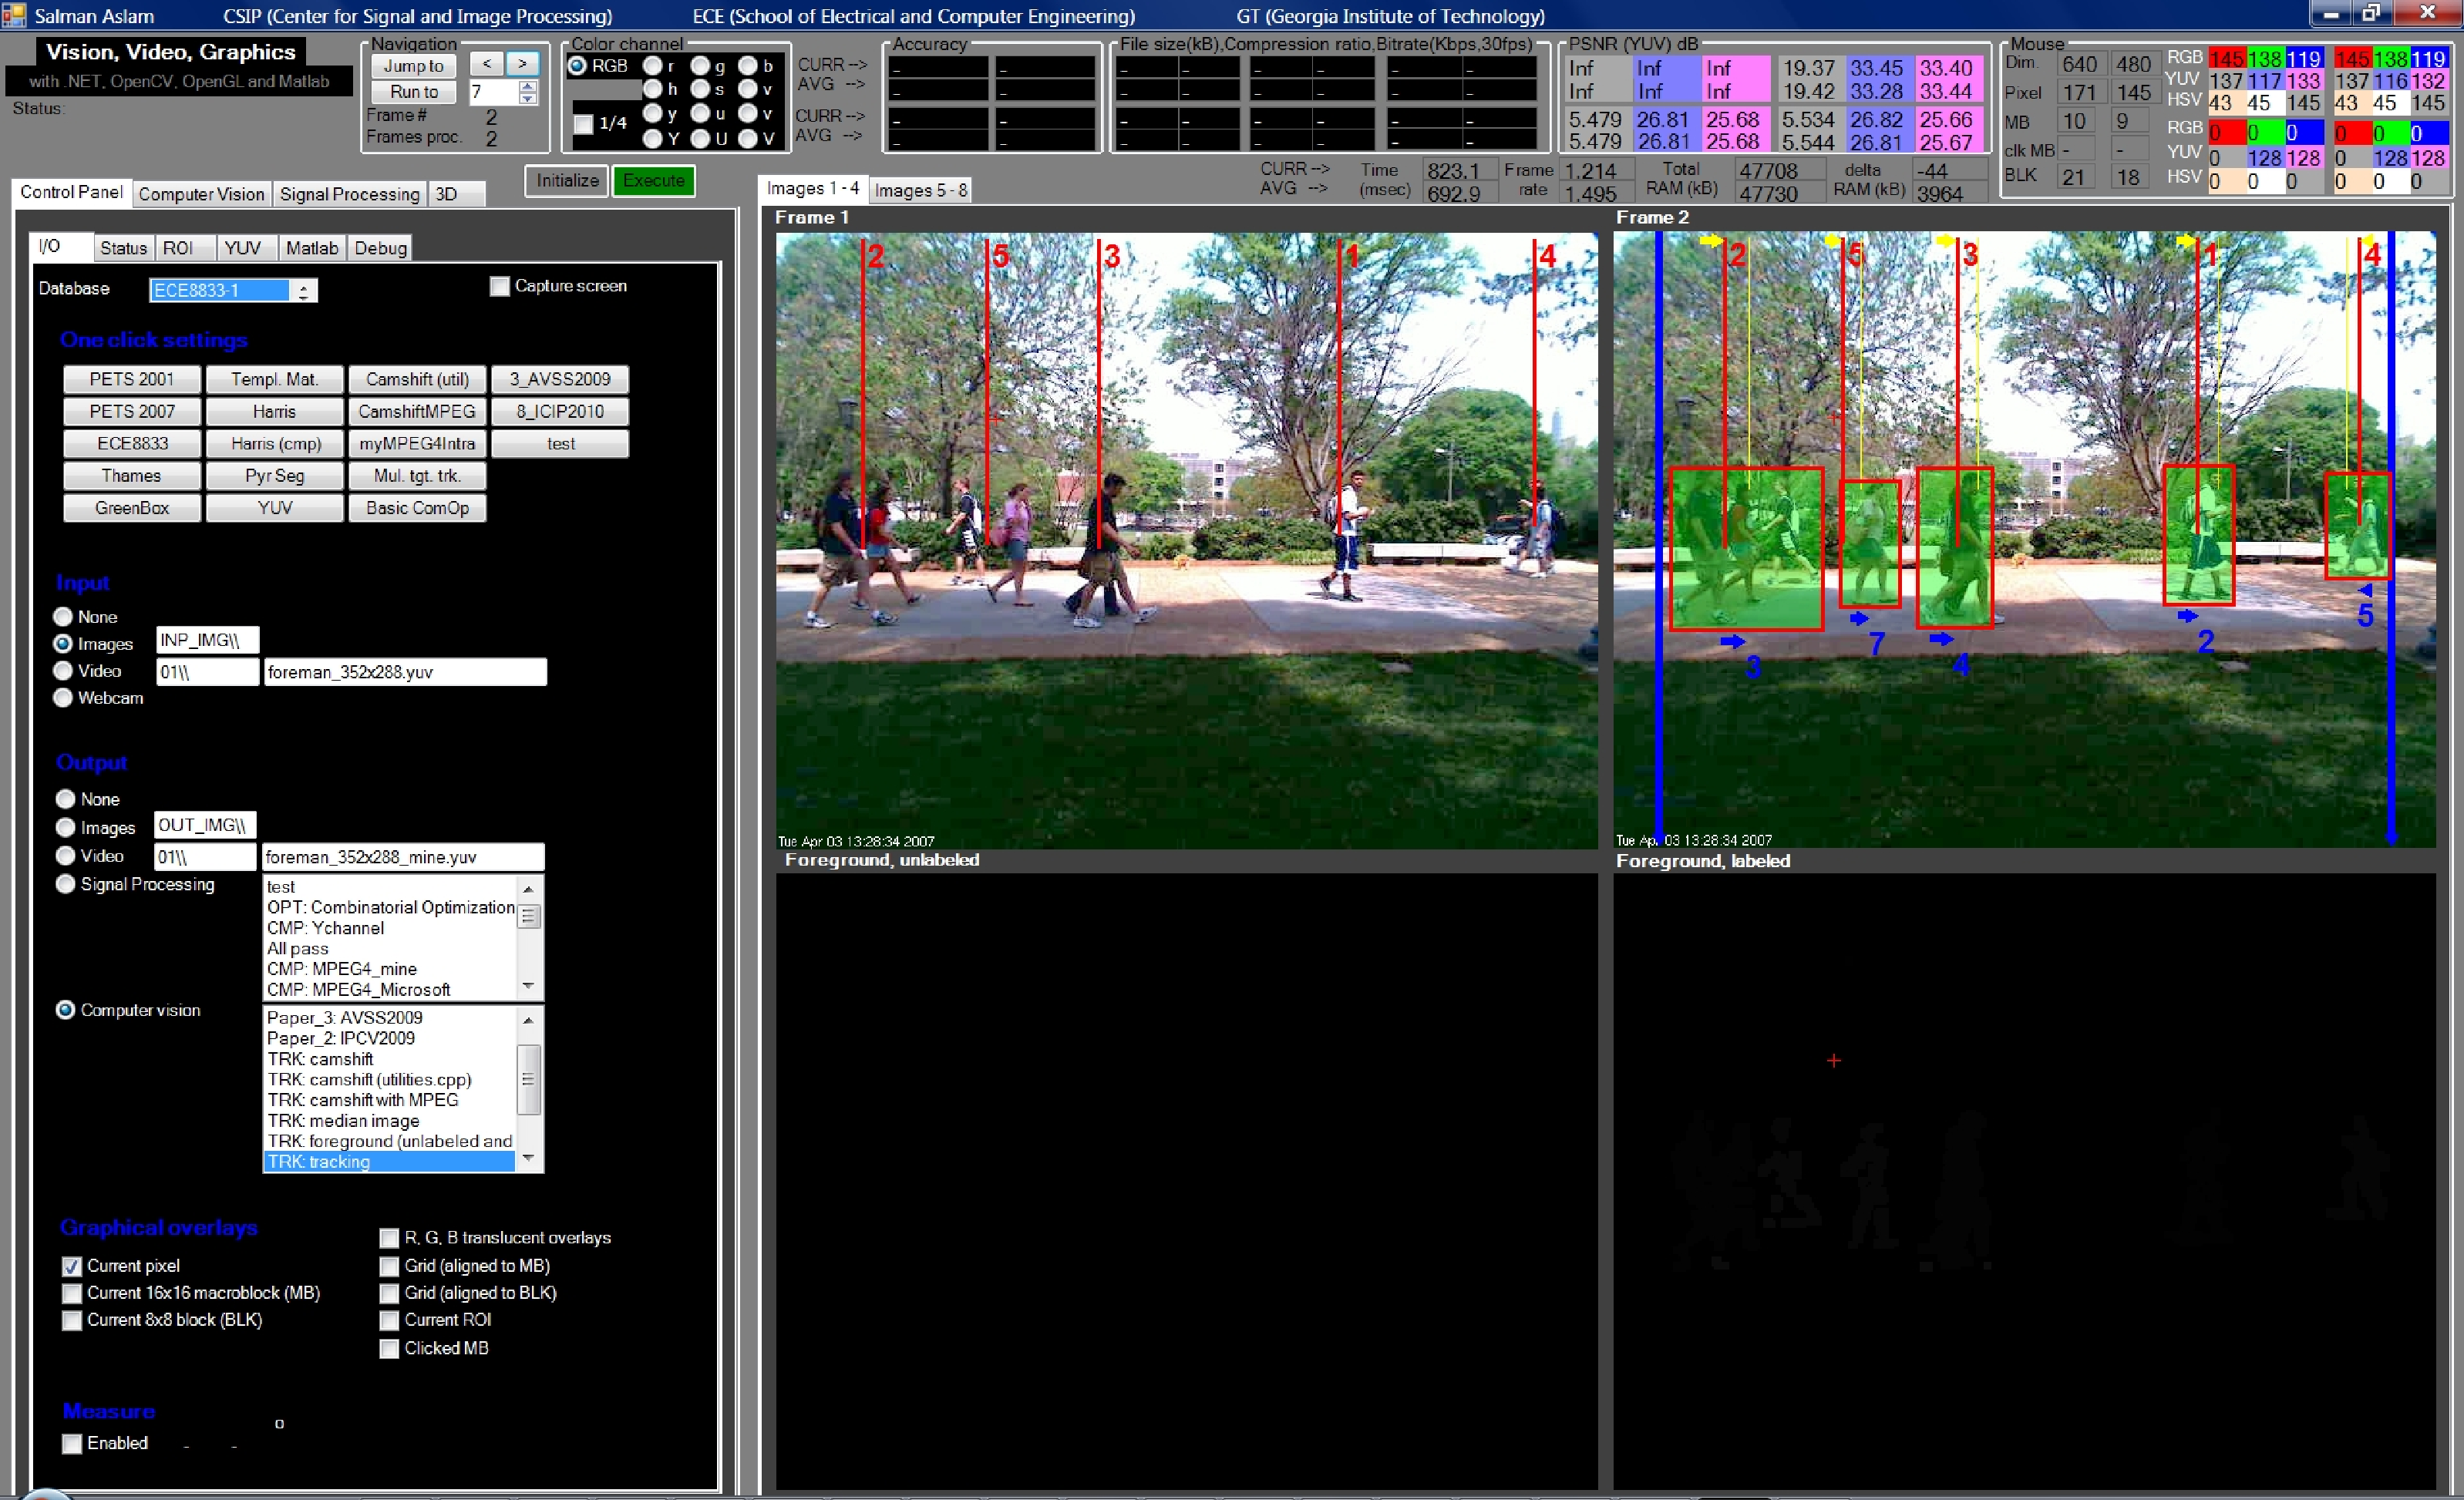
\includegraphics[width=0.8\textwidth]{figs/RVQ_TRK_IPCV2010_snapshot_VVG_ECE8833_FN_00002}
	\caption{Software.} 	
	\label{fig:snapshot_VVG}	
\end{figure*}

First, the $\sigma$-tree classifier is a type of variable rate vector quantizer \cite{2003_JNL_HighRateVQDetection_Hero}.  Second, Truncel \emph{et al} explore the relationship between rate-distortion theory and content-based retrieval in high dimensional databases \cite{2004_JNL_RateDistortionVsDatabases_Truncel}.  Third, the $\sigma$-tree design problem parallels the joint codebook design problem addressed in the source coding literature for multiple stage vector quantization \cite{1996_JNL_AdvancesRVQ_Barnes}.  Fourth, the $\sigma$-tree classifier can be compared to dimensionality reduction methods such as Principal Components Analysis (PCA).  PCA seeks to reorient the basis vectors in $\mathbb{R}^k$ and achieves compression by ignoring projected data components with least variances.  Even though a $\sigma$-tree classifier can be used to achieve lower dimensionality, it primarily seeks to partition $\mathbb{R}^k$ like other well known classifiers such as neural networks and support vector machines \cite{2007_JNL_IDDM_Barnes}.  Further, note that neural networks partition the decision space with hyperplanes or hypersurfaces, depending on whether or not hidden layers are used.  Support vector machines also do partition the decision space, but with hyperplanes in a higher dimension space that separate the data with maximum margin.  The $\sigma$-tree classifier tesselates the decision space $\mathbb{R}^k$ with $k$ Voronoi cells, the geometric dual of delaunay triangulation in $\mathbb{R}^2$.  The fifth and final comparison is with the well-known $k$-means algorithm, or the Linde Buzo Gray (LBG) algorithm as it is more commonly referred to in the source coding literature.  It is also called the Generalize Lloyd Algorithm (GLA).  Most vector quantization methods use this algorithm to create cluster centroids \cite{1991_BOOK_VQ_GershoGray}.  Indeed, the $\sigma$-tree classifier centroids can also be designed using this algorithm.  For a concrete and simple example of a $\sigma$-tree, see \cite{2007_JNL_IDDM_Barnes}.


The mechanism that allows a $\sigma$-tree to be built is multi-stage Vector Quantization (VQ), also called Residual Vector Quantization (RVQ) or Direct Sum Successive Approximation (DSSA) Vector Quantization.  These three terms will be used interchangeably in this paper.  Juang and Gray first proposed the RVQ structure \cite{1982_CNF_SpeechRVQ_JuangGray} and suggested that RVQ stages be designed by sequential application of GLA.  The main shortcoming of this approach is that each stage codebook is generated while considering only the error due to the previous stages (the \emph{causal error}); the error due to subsequent stages (the \emph{anticausal error}) is ignored.  A joint design approach on the other hand takes into account both the causal and anticausal errors to reduce the \emph{total error}.  Various techniques have been proposed for joint optimization.  We now introduce notation and define "joint optimality."

The $pth$ stage of a $P$-stage RVQ, with $N$ codevectors per stage, is a $k$-dimensional VQ defined by the mapping 
\begin{equation}
Q_p : \mathbb{R}^k \mapsto C_p
\end{equation}
  
Here, $\mathbb{R}^k$ is the $k$-dimensional input space,   

\begin{equation}
C_p = \{y_p(0), y_p(1), \ldots y_p(N_p - 1) \}
\end{equation}

is the $pth$-stage codebook and $y_p(i_p) \in \mathbb{R}^k$ is a $pth$-stage \emph{codevector}.  
Residual quantizer stage mappings $Q_p$ are collectively equivalent to a single mapping,

\begin{equation}
Q : \mathbb{R}^k \mapsto C
\end{equation}

\begin{figure}%[htp]
			\centering	
			\subfigure[Decoder codebooks.]
			{
				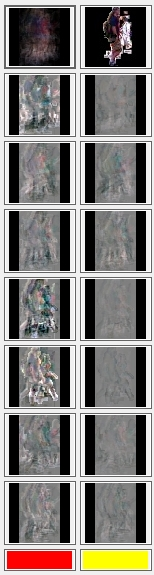
\includegraphics[width=0.10\textwidth]{figs/RVQ_TRK_IPCV2010_codebooks}
				\label{fig:Decoder_Codebooks}	
			}
			\subfigure[Reconstructing target using direct sum successive approximation templates.]
			{
				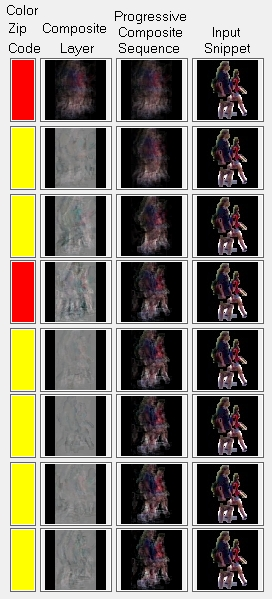
\includegraphics[width=0.20\textwidth]{figs/RVQ_TRK_IPCV2010_reconstruction}
				\label{fig:reconstruction}	
			}
			\caption{Using decoder codebooks to reconstruct targets.} 
			\label{fig:Codebooks_and_reconstruction}				
\end{figure}


Here, $C$ is the \emph{direct sum codebook} and is the direct sum of the stage codebooks $C=C_1 + C_2 + \ldots C_p$.  
In practice, the stage mappings $Q_p(.)$ are realized as a composition of a stage encoder mapping $E_p = \mathbb{R}^k \mapsto I_p$, and a stage decoder mapping $D_p: I_p \mapsto C_p$, that is $Q_p(x_1) = D_p[E_p(x_1)]$, where $x_1$ is a realization of $X_1$, which is the random source output.  


%The direct sum codebook is the direct sum of the stage codebooks $C=C_1 + C_2 + \ldots C_p$.  In practice, the stage mappings $Q_p$ %are realized as a composition of a stage encoder mapping $E_p: $
An RVQ is said to be jointly optimal if a local or global minimum value of the average distortion $d(E,D) = E[m(X_1, D(E(X_1)))]$ is achieved, where $m(.,.)$ is a distortion metric, and E[.] is the expectation operator.  This shows that an RVQ is a product code VQ with a direct sum codebook structure \cite{1993_JNL_RVQDSC_Barnes}.  Also notice that computation (search) and memory (storage) requirements are proportional to $kNP$.  So, the cost functional grows linearly with classifier dimensionality $k$, branch multiplicity $N$, and the number of tree levels $P$.  However, the number of indexing options is $N^P$.  This computational advantage makes it possible to use RVQ in real time tracking, even though the data dimensionality is very high.

%A near neighbor search is proportional in computational complexity to $MP$ whereas there is one of $M^P$ possible outcomes.
%Different types of VQ deal with how the partitions are created, indexed, or searched.  An RVQ is different from a traditional VQ in the sense that it partitions $\mathbb{R}^k$ into $M$ cells.  The residual space, also in $\mathbb{R}^k$, is then partitioned again into $M$ cells.  This process is repeated $P$ times.  The advantage of this approach is that in obtaining $M^P$ partitions, we need to run our partitioning algorithm $P$ times and generate $M$ partitions at each stage.  In traditional VQ, the partitioning algorithm would run once but have to create $M^P$ partitions.  For the binary case, i.e. two templates per stage, $M=P$, and if 8 stages are used, we require only 16 searches, whereas in traditional VQ, this would require 256.  

%--------------------------------------------------------------------------------------------------------------------------------------
\subsection{Background Subtraction}
%--------------------------------------------------------------------------------------------------------------------------------------
Several preprocessing steps may be required before tracking can be initiated.  These could include image stabilization, normalization, and downsampling.  The final preprocessing step in most cases is background modeling.  Several algorithms have been developed for this task.  Most of these algorithms depend on appearance modeling.  A detailed overview alongwith a graphical comparison of how these algorithms perform on the canonical problems in foreground detection is given in \cite{1999_CNF_Wallflower_Toyama}.  In this paper, we use the Multi Gaussian algorithm~\cite{2000_JNL_MG_Stauffer}.  In this algorithm, the grayscale value of each pixel is tracked over time and represented as a mixture of $K$ Gaussian distributions.  The mean and variance of the Gaussians is tracked over time.  This is a pixel based approach with no region based processing.  However a post processing step of morphological operations, connectedness constraints, and area thresholding makes the combined approach quite robust to slow drifts in appearances.  The probability of observing the current pixel value at time, $x_t$, is 

\begin{equation}
p(x_t)=\sum_{i=1}^{K}\omega_{i,t}*\eta(X_t, \mu_{i,t}, \Sigma_{i,t})
\end{equation}

where $K$ is the number of distributions,  $\omega_{i,t}$ is an estimate of the weight of the $i$th Gaussian in the mixture at time $t$.  The gaussian distributions are given by,

\begin{equation}
\eta(x_t, \mu, \Sigma)=\frac{1}{(2\pi)^\frac{n}{2}|\Sigma|}e^{-\frac{1}{2}(X_t-\mu_t)^T\Sigma^{-1}(X_t-\mu_t)}
\end{equation}

  The pixel process is not stationary, and so one cannot resort to maximizing the likelihood of the observed data using the Expectation Maximization (EM) algorithm.  Instead, the weights of the Gaussians are adjusted as follows,

\begin{equation}
\omega_{k,t} = (1-\alpha) \omega_{k,t-1} + \alpha M_{k,t}
\end{equation}

where $\alpha$ is the learning rate, and $M_{k,t}$ is 1 for the model which matched and 0 otherwise.  A match is defined as a pixel within 2.5 standard deviations of a distribution.  In this paper, we use a value of $K=3$. 

%%--------------------------------------------------------------------------------------------------------------------------------------
%\subsection{Tracking}
%%--------------------------------------------------------------------------------------------------------------------------------------
%Multi-target tracking is a complex, but well studied problem.  \cite{2006_JNL_TrackingSurvey_MubarakShah} provides a comprehensive overview of this area.  
%The problem can be further compounded if a perspective projection is used.  During initialization, every observation can be assigned a target.  In the absence of velocity information, a state estimation algorithm such as the Kalman or Particle Filter cannot be initialized.  Maintaining multiple hypotheses In subsequent frames, To reduce the combinatorial possibilities of target location in the subsequent frames during this training period, the number of possible directions can be quantized to a limited number of levels.    Therefore, in order to reduce the complexity of the comThe number of possible directions that the target can move in can be quantized to reduce the possibilities of where the targets could be in the next frame.  In the absence of velocity information,   Tracks are initialized at frame 0.  In the 2D tracking case in which 

%%--------------------------------------------------------------------------------------------------------------------------------------
%\section{Particle Filter}
%%--------------------------------------------------------------------------------------------------------------------------------------
%The particle filter is a powerful tool in Bayesian estimation if the system is non-linear and/or the noise is non-Gaussian.  In such cases, the (Extended) Kalman Filter may exhibit poor performance [11].  In this case, one is forced to look beyond the Kalman filter.  The particle filter is a popular mechanism employed in such cases although its main disadvantage is its computational load.  
%Consider the standard filtering formulation
%Here, xk   Rn is the state vector of the system, a, b: RnxR Rn and c: RnxR Rm are vector valued functions.  wk is the process noise, vk is the measurement noise, and they are both white sequences with known distribution. po(x) is a known distribution for the initial state xo.  Furthermore, it is assumed that wk, vk and xo are independent.  Zk := {z1, z2, � } is the observation vector.  Then, when an observation arrives, i.e. a realization of Zk, the filtering problem is to find the best estimate of x given Zk.  In the linear Gaussian case, p(xk|Zk) is also Gaussian and the Kalman filter provides an optimal closed form solution.  In the non-linear and/or non-Gaussian case, the Kalman filter may not provide an adequate solution.  Using Bayes' Rule, it is known that,
%
%            (5)
%The Kalman filter is a closed form solution for the above equation for the linear Gaussian case.  An approximate solution is the so called sampling filter approach.  The core of the sampling filter algorithm is that the above equation is approximated on the basis of an N point grid in the state space [12].  
%
%The basic idea behind the particle filter is that we represent the posterior distribution of interest with a set of weighted particles, each of which forms an independent hypothesis of the state at a given time [13].  The weights have to be chosen correctly for this weighted set of particles to be representative of the posterior distribution.  To get an estimate of the state, MAP or MMSE estimates can be used, although in our experience, the MAP estimate tends to work better.  In the first step, a set of particles from the previous time step are used to propose a new setup for the new time step.  In the second step, these are weighted to ensure consistency.  Finally, the weighted particles are resampled to convert them into an unweighted set without changing the distribution they represent.  

%--------------------------------------------------------------------------------------------------------------------------------------
\section{EXPERIMENTS}
%--------------------------------------------------------------------------------------------------------------------------------------
We track multiple targets using multi-stage, direct sum successive approximation RVQ.  A block diagram of our approach is shown in Figure~\ref{fig:block_diagram} while a sample tracking scenario is shown in Figure~\ref{fig:snapshot_VVG}.  We track several targets in a dense environment.  Background maintenance is done using a Multi Gaussian background subtraction algorithm.  Tracking intialization is done using template matching.  When enough training examples of a particular target have been attained, they are input into a multi stage residual vector quantizer to train the encoder and decoder codebooks.  During the bootstrapping process, this process is repeated for all targets.  Subsequent foreground objects are tested against the codebooks of every target.  The codebook that most explains the target is chosen.  This is equivalent to Probabilistic Multiple Hypothesis Testing (PMHT) with hard decisions.  In subsequent work, we will demonstrate soft decisions alongwith temporal evolution of the codebooks in real-time.  In this paper, we limit ourselves to demonstrating the effectivness of using RVQ in the multi-target tracking scenario.

For this purpose, we have developed the software shown in Figure~\ref{fig:snapshot_VVG}.  It is integrated with Matlab and Intel OpenCV for basic mathematical, image processing and visualization purposes.  Where more elaborate 3D visualization is required, for instance in viewing error surfaces, where each point on the surface corresponds to a pixel in an image, OpenGL is used for rendering a height map over the texture mapped image. The software GUI is developed in Visual Studio.NET.

%--------------------------------------------------------------------------------------------------------------------------------------
\section{RESULTS}
%--------------------------------------------------------------------------------------------------------------------------------------
Figure~\ref{fig:Decoder_Codebooks} shows the direct sum templates of the decoder codebook.  We use 2 codevectors per stage ($N=2$), and a total of 8 stages ($P=8$).  Although this number is somewhat arbitrary, empirical analysis shows this to be a reasonable setting.  A total of $N^P$, or 256 unique images can be represented with this codebook, but the computational cost of computation and storage is $O(NP)$ rather than $O(N^P)$.  Once the codebooks have been created for time $t=1$ to $t=T$, subsequent targets at times $t=T+1, T+2, \ldots$ are encoded using the codebooks.  The codebook that results in the least reconstruction error is chosen and the target corresponding to that codebook is matched.  Figure~\ref{fig:reconstruction} shows reconstruction of a target using the codebooks.  In Figure~\ref{fig:PSNR_3D} we show the PSNR value of target reconstruction in a window centered around the target.  PSNR values are low if the target under test and the codebooks being used are mismatched.  However, if they are matched, the PSNR is sufficiently high for unambiguous correspondence.  This is shown in tabular form in Table~\ref{fig:Table} where PSNR values at the center of the targets are reported. 


\begin{figure}
			\centering
			\subfigure[For a given codebook $C_i$, a target from within the training set used to generate $C_i$ produces a high PSNR as compared to targets that do not belong to the training set.]
				{
				\label{fig:training}	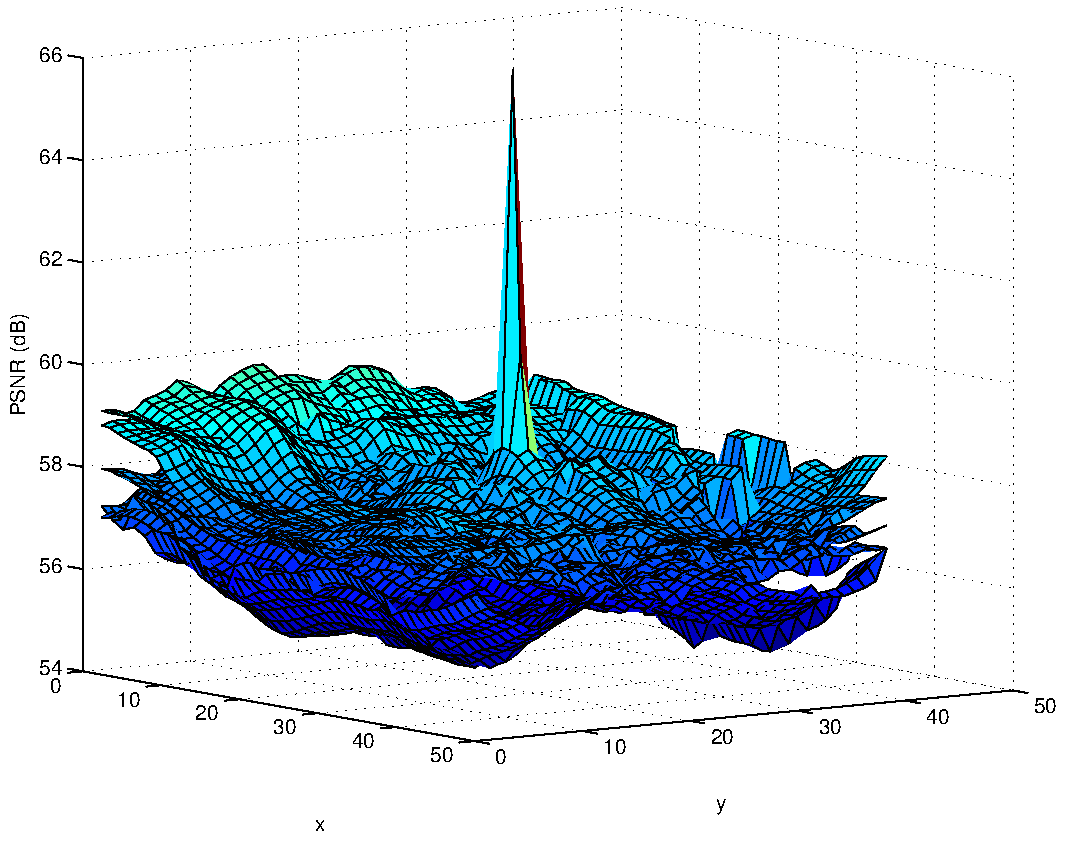
\includegraphics[width=.45\textwidth]{figs/RVQ_TRK_IPCV2010_CODEBOOK_tgt2_PROJECTION_tgt1_frame7_tgt_2_frame7_tgt3_frame7_tgt5_frame7_tgt9_frame33}
				}
%			\subfigure[Target 5 codebook.]
%				{	\includegraphics[width=.45\textwidth]{figs/CODEBOOK_tgt5_PROJECTION_tgt1_frame7_tgt_2_frame7_tgt3_frame7_tgt5_frame7_tgt9_frame33.eps}
%				}
%			\subfigure[Target 9 codebook.]
%				{	\includegraphics[width=.45\textwidth]{figs/CODEBOOK_tgt9_PROJECTION_tgt1_frame7_tgt_2_frame7_tgt3_frame7_tgt5_frame7_tgt9_frame33.eps}
%				}	
			\subfigure[Here the target under test was not used to generate the codebook $C_i$.  Nevertheless, it belongs to the same class as $C_i$ but is 3 frames temporally advanced, i.e. $t=T+3$ where $C_i$ was generated over $t=1 \ldots T$.  Notice that it still has significantly higher PSNR than targets outside the class.]
				{
					\label{fig:testing}	
					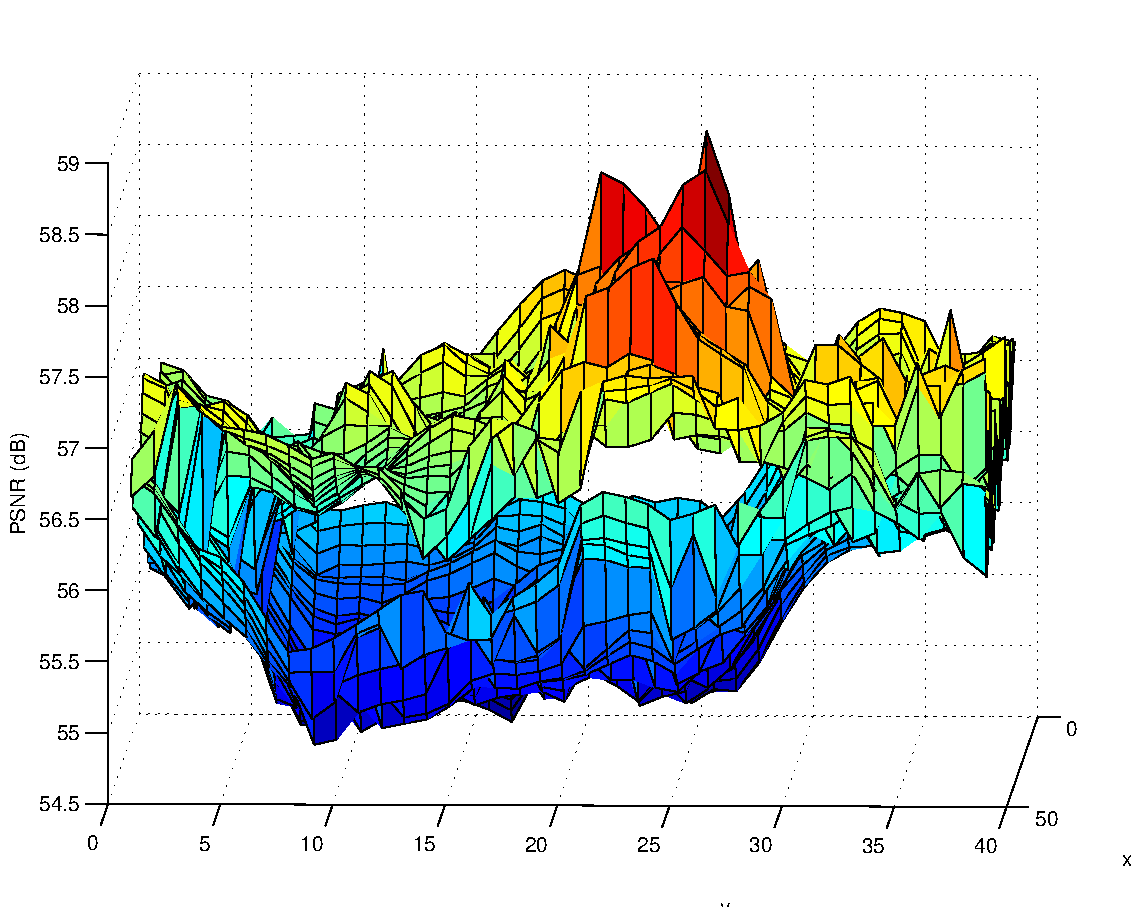
\includegraphics[width=.45\textwidth]{figs/RVQ_TRK_IPCV2010_reconstructionPSNR}
				}		
		\caption{Computing PSNR for target reconstruction.} 					
		\label{fig:PSNR_3D}	
\end{figure}






\begin{figure}
		
	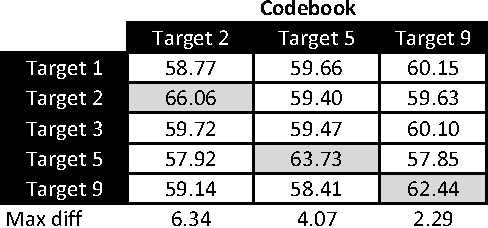
\includegraphics[width=0.50\textwidth]{figs/RVQ_TRK_IPCV2010_resultsTable}
	\caption{Maximum PSNR values, in dB, of all targets for given codebooks.  Also shown is the difference between the two highest PSNR values. } 	
	\label{fig:Table}
	\end{figure}

%--------------------------------------------------------------------------------------------------------------------------------------
\section{CONCLUSIONS}
%--------------------------------------------------------------------------------------------------------------------------------------
We demonstrate the first reported application of residual vector quantization to any form of video processing.  In this paper, the application we focus on is multi-target tracking.  We demonstrate initial results of a completely automatic method of training RVQ encoder and decoder codebooks, and then using them to detect targets.  We show that this method can track targets in a difficult multi-target tracking scenario.  In future work, we will focus on temporal evolution of the codebooks to generate time evolving desriptions of the targets under test.

%--------------------------------------------------------------------------------------------------------------------------------------
%BIBLIOGRAPHY
%--------------------------------------------------------------------------------------------------------------------------------------
\bibliographystyle{IEEE}
\bibliography{MyCitations}
\end{document}
